\section{Projektmanagement Planung}
Für die Organisation des Projektes wurde der webbasierte Hosting-Dienst
Github verwendet. Auf einem über Github erstellten Verzeichnis (Repository
genannt) werden alle relevanten Daten fürs Projekt zentral gespeichert und
sind so für alle Teammitglieder über das Internet ständig zugänglich. Die
Verwaltung der Daten erfolgt über ein gleichnamiges Programm oder direkt
über das verteilte Versionsverwaltungssystem Git. Werden Änderungen an
einer Datei vorgenommen, wird diese vom Programm erkannt und kann vom
Benutzer anschliessend commited (Bestätigung zur Übernahme der Änderung)
werden. Arbeiten zwei Teammitglieder gleichzeitig an der selben Datei
entsteht ein Konflikt, welcher in einem Merge-Prozess (Zusammenführen)
aufgelöst wird. Diese Konflikte lassen sich grösstenteils durch eine gute
Organisation und Arbeitsteilung vermeiden.

Mittels Github können sogenannte \emph{Issues} verwaltet werden. Diese
\emph{Issues} beschreiben jeweils eine konkrete Aufgabe. Diese können
einem Teammitglied zugewiesen werden, besitzen einen Status (offen,
erledigt) und werden zeitlich terminiert in dem sie einem
\emph{Meilenstein} zugewiesen werden. Diese \emph{Issues} ermöglichen
es so, die Aufgaben einfach und effektiv zu verteilen.

Die Aufgabenstellung dieses Projektes beinhaltete die Abgabe von 3
Berichten über den Verlauf des Semesters hinweg. Mittels Github wurde
für jede Abgabe jeweils ein \emph{Meilenstein} erstellt, welcher die
zu erledigenden Aufgaben bzw. \emph{Issues} für die Berichte
zusammenfasst. So weiss jeder Nutzer jeweils Bescheid was er bis zur
Abgabe zu tun hat.

\subsection{Kostenübersicht}
Für unseres Projekt hatten wir ein Budget von 600.00 CHF. Die Kosten
wurden in einer Tabelle verwaltet um den Überblick zu wahren. Die
Schätzung für die Kosten wurden in der Kolonne Budget eingetragen. Die
Schätzung des Budget basiert auf Recherchen im Internet und sind jeweils
mit den maximal Kosten budgetiert. Aus dies ist anzunehmen, dass eher
weniger gebraucht wird, als budgetiert.

\begin{figure}[h!]
	\center
	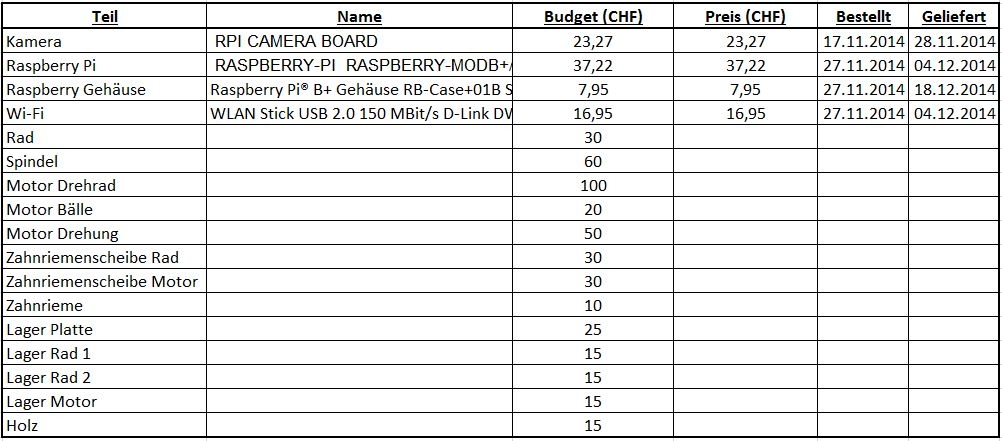
\includegraphics[width=0.8\textwidth]{../../fig/Kostenuebersicht.jpg}
	\caption{Kostenübersicht}
	\label{fig:Kostenuebersicht}
\end{figure}

Das gesamt Budget des PREN-Projekts liegt bei 600.00 CHF. Bisher rechnen
wir damit, dass 500.00 CHF für ein erfolgreiches umsetzen reichen sollten.
Die restlichen 100.00 CHF dienen als gute Reserve für das Korrigieren von
Fehlentscheidungen. Im PREN 1 durfte 200.00 CHF ausgegeben werden, davon
wurde 85.40 CHF gebraucht. 

\subsection{Projekteam}

\begin{tabularx}{\columnwidth}{XX}
	
	\textbf{Adriano Valsangiacomo} \newline
	Maschinentechnik \newline
	\href{mailto:adriano.valsangiacomo@stud.hslu.ch}{adriano.valsangiacomo@stud.hslu.ch} \newline
	
	&  
	
	\textbf{Ervin Mazlagi\'c} \newline
	Elektrotechnik \newline
	\href{mailto:ervin.mazlagic@stud.hslu.ch}{ervin.mazlagic@stud.hslu.ch} \newline 
	
	\\ 
	
	\textbf{Christian Spycher} \newline
    Maschinentechnik \newline
    \href{mailto:christian.spycher@stud.hslu.ch}{christian.spycher@stud.hslu.ch} \newline 
     
    
    & 
    
    \textbf{Fabian Wüthrich} \newline
    Informatik \newline
    \href{mailto:fabian.wuethrich.01@stud.hslu.ch}{fabian.wuethrich.01@stud.hslu.ch} \newline 
    
    \\ 
	
	\textbf{Christian Schürch} \newline
	Maschinentechnik \newline
	\href{mailto:christian.schuerch@stud.hslu.ch}{christian.schuerch@stud.hslu.ch} \newline 
	
	& 
	 
	\textbf{Alexander Suter} \newline
	Informatik \newline
	\href{mailto:alexander.suter@stud.hslu.ch}{alexander.suter@stud.hslu.ch} \newline 
	
	\\ 
\end{tabularx} 


\subsection{Organigramm}
Die Hierarchie des Projektteams ist im Organigramm in Abbildung \ref{fig:organigramm} dargestellt.

\begin{figure}[h!]
	\centering
	\begin{tikzpicture}
	\node [draw](projektleiter) {
		\begin{tabular}{c}
		Projektleiter \\
		Adriano \\
		Valsangiacomo
		\end{tabular} 
	};
	
	\node [draw, below left =1cm and 2cm of  projektleiter] (informatik) {Informatik} edge [<-] (projektleiter);
	\node [draw, below =1cm of  projektleiter] (elektrotechnik) {Elektrotechnik} edge [<-] (projektleiter);
	\node [draw, below right =1cm and 2cm of  projektleiter] (mechanik) {Mechanik} edge [<-] (projektleiter);
	
	\node [draw, below left  = of  informatik] (fabianwuethrich) {
			\begin{tabular}{c}
			Fabian \\
			Wüthrich
			\end{tabular}
		} edge [<-] (informatik);
	\node [draw, below right = of  informatik] (alexsuter) {
			\begin{tabular}{c}
			Alexander \\
			Suter
			\end{tabular} 
		} edge [<-] (informatik);
	
	\node [draw, below =3cm of  elektrotechnik] (ervinmazlagic) {
			\begin{tabular}{c}
			Ervin \\
			Mazlagi\'c
			\end{tabular}
		} edge [<-] (elektrotechnik);
	
	\node [draw, below left = of  mechanik] (christianspycher) {
		\begin{tabular}{c}
		Christian \\
		Spycher
		\end{tabular} 
		} edge [<-] (mechanik);
	\node [draw, below = of  mechanik] (christianschuerch) {
		\begin{tabular}{c}
		Christian \\
		Schürch
		\end{tabular}} edge [<-] (mechanik);
	\node [draw, below right = of  mechanik] (adrianovalsangiacomo) {
				\begin{tabular}{c}
				Adriano \\
				Valsangiacomo
				\end{tabular}  
		  } edge [<-] (mechanik);
	\end{tikzpicture}
	\caption{Organigramm}
	\label{fig:organigramm}
\end{figure}


\begin{landscape}
\section{Risikoanalyse}
\begin{table}[h!]
    \centering
    \begin{tabular}{p{0.1\textwidth} c p{0.15\textwidth} p{0.2\textwidth} p{0.15\textwidth} p{0.1\textwidth} p{0.2\textwidth}}
		& Nr. & Risiko & Ursache & Wahrscheinlichkeit & Auswirkung & Massnahmen \\
        \hline \hline
        & & & & & & \\
        \rowcolor{yellow} 
        Personelle Faktoren & 1 & Falscher Projektleiter & Falsche Vorstellungen vom Projekt & Vorstellbar & gering & Erfolg darf nicht vom Projektleiter abhängen \\ 
        \rowcolor{yellow}
	    & 2 & Zwei Mitglieder einer Studienrichtung fallen aus & Krankheit, Studienabbruch & Unwahrscheinlich & Katastrophal & externe Hilfe holen \\
        \rowcolor{green}
        & 3 & Betreuender Dozent fällt aus & Krankheit, beschäftigt mit anderen Projekten & vorstellbar & unwesentlich &
	\end{tabular}
\end{table}
\end{landscape}


\subsection{Risiko-Bewertungsschema}
\begin{table}[h!]
	\renewcommand{\arraystretch}{1.5}
	\centering
	\begin{tabular}{r || c c c c}
		häufig 		
			& \cellcolor{red} 
			& \cellcolor{red}
			& \cellcolor{red}
			& \cellcolor{red} \\
		wahrscheinlich		
			& \cellcolor{yellow} 
			& \cellcolor{yellow} 
			& \cellcolor{red}
			& \cellcolor{red} \\
		gelegentlich		
			& \cellcolor{yellow}
			& \cellcolor{yellow}
			& \cellcolor{yellow}
			& \cellcolor{red} \\
		vorstellbar		
			& \cellcolor{green}
			& \cellcolor{yellow}
			& \cellcolor{yellow}
			& \cellcolor{yellow} \\
		unwahrscheinlich	
			& \cellcolor{green}
			& \cellcolor{green}
			& \cellcolor{yellow}
			& \cellcolor{yellow} \\
		unvorstellbar		
			& \cellcolor{green}
			& \cellcolor{green}
			& \cellcolor{green}
			& \cellcolor{green} \\
		\hline
		& unwesentlich & geringfügig & kritisch & katastrophal
	\end{tabular}
\end{table}

